\chapter{Requisitos do Sistema}

\section{Requisitos Funcionais}

% Apresentar os requisitos funcionais, que especificam a��es que o sistema deve ser capaz de executar, ou seja, as fun��es do sistema. Classifique as funcionalidades quanto a prioridade: 
% Essencial ? deve ser implementado para que o sistema funcione. 
% Importante ? sem este requisito o sistema pode funcionar, mas n�o da maneira esperada.
% Desej�vel ? este tipo de requisito n�o compromete o funcionamento do sistema.

\begin{center}
	\begin{tabular}{ | C{1cm} | m{11.7cm}| m{2.3cm} | } 
		\hline
		\textbf{ID} & \textbf{Funcionalidade} 							& \textbf{Prioridade} \\ \hline
		RF1 		& Salvar inteiros, floats, booleans e strings. 		& Essencial \\ \hline
		RF2 		& Carregar inteiros, floats, booleans e strings. 	& Essencial \\ \hline
		RF3 		& Usar o Facebook para realizar login. 				& Essencial \\ \hline
		RF4			& Suportar m�ltiplos jogos. 						& Essencial \\ \hline
		RF5			& Gerar Leaderboards a partir dos inteiros.			& Importante \\ \hline
		RF6			& Sistema de achievements.							& Desej�vel \\ \hline
	\end{tabular}
\end{center}

\section{Requisitos N�o-Funcionais}

% Descrever os requisitos n�o-funcionais do sistema, que especificam restri��es sobre os servi�os ou fun��es providas pelo sistema, categorizando de acordo com a caracter�stica envolvida, como: Usabilidade, Padroniza��o, Ambiente, Compatibilidade, Recursos, etc.

\begin{center}
	\begin{tabular}{ | C{1cm} | m{11.7cm}| m{2.3cm} | } 
		\hline
		\textbf{ID} & \textbf{Requisito}												& \textbf{Categoria} \\ \hline
		RNF1 		& O sistema deve ser configur�vel atrav�s de vari�veis de ambiente.	& Usabilidade \\ \hline
		RNF2 		& Save deve ser feito em uma requisi��o ao servidor. 				& Usabilidade \\ \hline
		RNF3 		& Load deve ser feito em uma requisi��o ao servidor. 				& Usabilidade \\ \hline
		RNF4 		& Os Leaderboards devem ficar no cache por 120 segundos. 			& Usabilidade \\ \hline
	\end{tabular}
\end{center}

\pagebreak

\section{Diagramas de Casos de Uso}

% Inclua aqui os diagramas de Casos de Uso desenvolvidos para o sistema, usando os IDs dos itens anteriores como refer�ncia quando necess�rio.

\begin{figure}[ht!]
	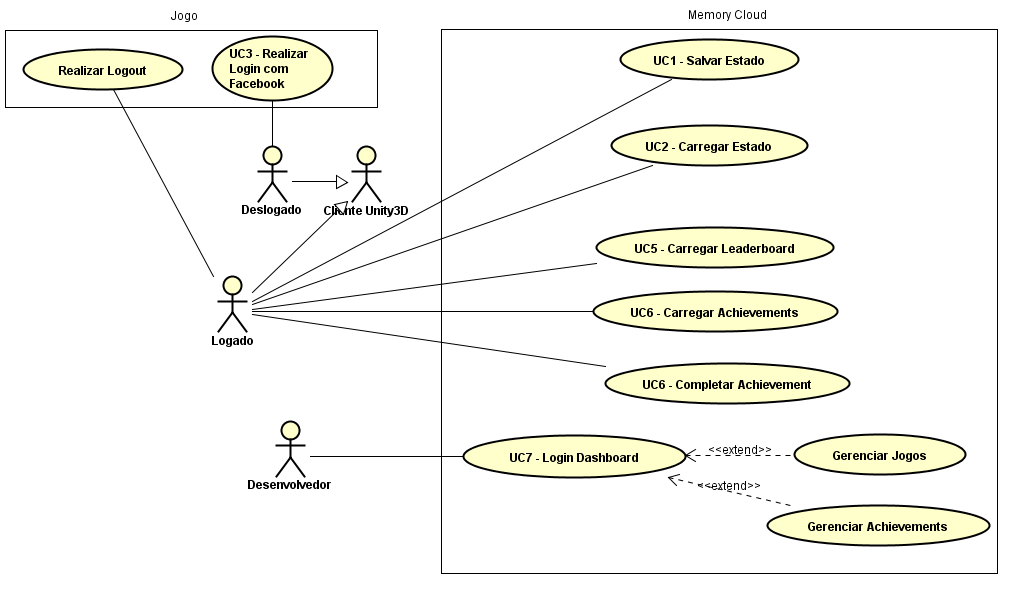
\includegraphics[width=\textwidth]{./4/casodeuso.png}
\end{figure}
